\documentclass[oneside,final,14pt]{extreport}
\usepackage[utf8]{inputenc}
\usepackage[T2A]{fontenc}
\usepackage[russian]{babel}
\usepackage{vmargin}
\setpapersize{A4}
\setmarginsrb{2cm}{1.5cm}{1cm}{1.5cm}{0pt}{0mm}{0pt}{13mm}
\usepackage{indentfirst}
\sloppy
\setcounter{secnumdepth}{3}
\setcounter{tocdepth}{3}
\usepackage{color}
\newcommand\marker[2]{{\fboxsep=0pt\colorbox{#1}{\strut #2}}}
\usepackage{graphicx}
\usepackage{amsmath}
\usepackage{animate}
\usepackage{hyperref}
\usepackage{listings}
\lstset{
    language = python, 
    frame=single, 
    captionpos = b,
    numbers = left,
    basicstyle=\footnotesize
}

\newcommand\chap[2]{
    \section*{#1}
    \addcontentsline{toc}{chapter}{#1}
}


\begin{document}

\begin{titlepage}
    \begin{center}
        \large
        МИНИСТЕРСТВО ОБРАЗОВАНИЯ И НАУКИ РОССИЙСКОЙ ФЕДЕРАЦИИ
        
        Федеральное агентство по образованию

        "<Пермский национальный исследовательский политехнический университет">
        
        Кафедра микропроцессорных средств автоматизации
        \vfill

        Отчёт по лабораторной работе \textnumero 2
        
        По дисциплине компьютерная графика
        
        На тему: "<Построение динамических изображений">
      
    \end{center}
    \vfill
   
    \newlength{\ML}
    \settowidth{\ML}{«\underline{\hspace{0.7cm}}» \underline{\hspace{1.5cm}}}
    \hfill
    \begin{minipage}{0.5\textwidth}
        Работу выполнили\\
        студенты гр. ИСУП-18-2м\\
        \underline{\hspace{\ML}} А.\,С.~Морозов\\
        \underline{\hspace{\ML}} В.\,О.~Раскошинский\\
    \end{minipage}%
    \bigskip
   
    \hfill\begin{minipage}{0.5\textwidth}
        Проверил доцент кафедры МСА\\
        \underline{\hspace{\ML}} Л.\,А.~Мыльников\\
    \end{minipage}%
    \vfill
   
    \begin{center}
        Пермь, 2020 г.
    \end{center}
\end{titlepage}

\newpage

\chap{Алгоритм морфинга}

Морфинг -- технология в компьютерной графике, визуальный эффект, создающий впечатление плавной трансформации одного объекта в другой. Встречается в трёхмерной и двумерной (как растровой, так и в векторной) графике.

Особенностью технологии морфинга является необходимость установления соответствия между точками исходного и конечного изображений.

\chap{Морфинг растровых изображений}

При работе с растровыми изображениями необходимо, чтобы разрешения исходного изображения и конечного совпадали. Тогда каждая точка исходного изображения становится в соответствие каждой точке конечного изображения, и работа алгоритма будет состоять в плавном преобразовании цвета по формуле:

\begin{equation}
  \label{morf:1}
  c = c_1 + (c_2 - c_1) \cdot t,
\end{equation}

\noindent где $0<t<1$ -- фаза морфинга, $c_1$ и $c_2$ -- цвета точки первого и второго изображений. Такая операция выполняется для каждой составляющей цвета в RGB или CMYK. 

Реализация алгоритма морфинга для растровых изображений представлена в листинге \ref{code:morf:rastr}. Результаты работы алгоритма представлены на рисунке \ref{morf:galkin}.

\begin{lstlisting}[caption = Реализация алгоритма морфинга для растровых изображений, label = code:morf:rastr]
from PIL import Image
import numpy as np

im1 = Image.open('1.png')
im2 = Image.open('2.png')

while True:
    n = input('enter the number of intermediate stages\n')
    try:
        n = int(n)
        break
    except:
        print('the number of intermediate stages is an integer')
        continue

pix_1 = np.array(im1)
pix_2 = np.array(im2)
pix_0 = np.zeros((n,) + pix_1.shape, dtype = int)

m = np.linspace(0, 1, num = n + 2)[1:-1] # num = number of frames + 2

iint = np.vectorize(int) # vectorize int

# morphing for all intermediate stages
for i in range(len(m)):
    pix_0[i] = iint(iint(pix_1) + (iint(pix_2) - iint(pix_1)) * m[i])
    
pix = np.hstack((pix_1, *pix_0, pix_2)).astype(np.uint8) # list of images
Image.fromarray(pix).show()
Image.fromarray(pix).save('gradient.png')
\end{lstlisting}

\begin{figure}[htb]
    \label{morf:galkin}
        \begin{center}
            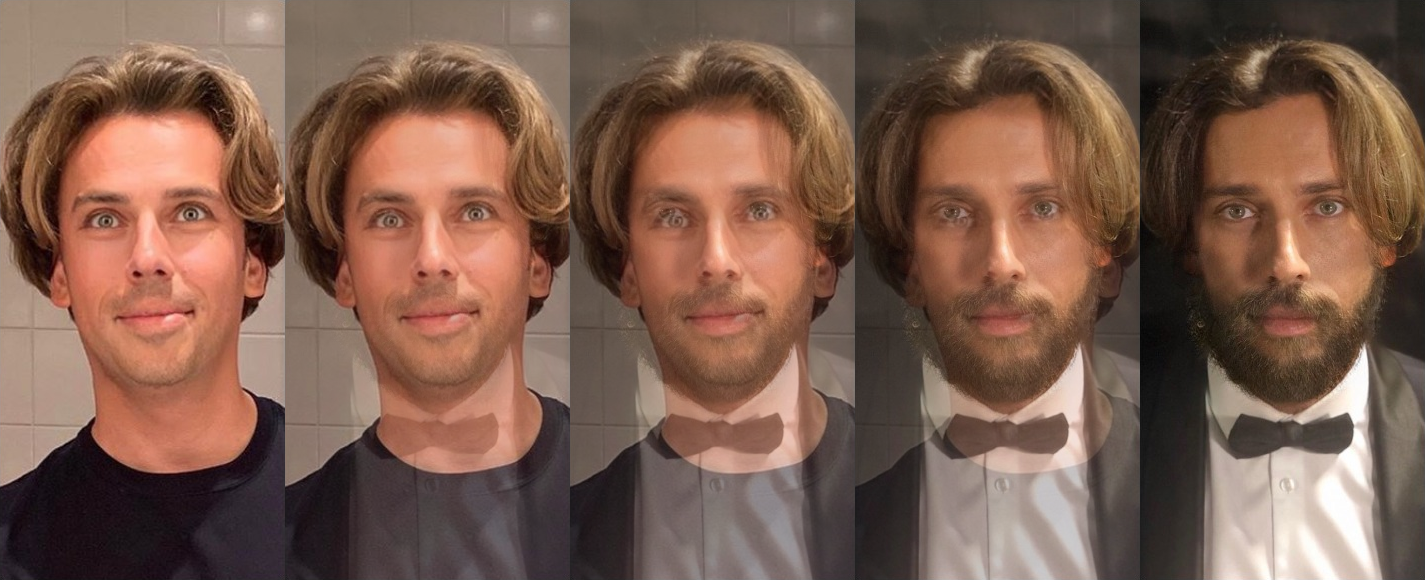
\includegraphics[width=\linewidth]{../face_morphing/gradient}
        \end{center}
    \caption{Результаты работы алгоритма морфинга для растровых изображений}
\end{figure}

\chap{Морфинг векторных изображений}

При использовании векторной графики устанавливается соответствие между точками исходного и целевого изображения. Таким образом получаем пары значений $\left(y_1^{(0)},x_1^{(0)}\right),\left(y_1^{(1)},x_1^{(1)}\right)$ и т.д. в зависимости от количества промежуточных состояний и точек изображений. Для изменения значений координат обычно используется уравнение прямой $(y = a + b \cdot x)$, но могут использоваться и другие фигуры, описываемые аналитически. Зная две координаты, мы можем определить значения коэффициентов $a$ и $b$ из системы уравнений

\begin{equation*}
    \left\{
        \begin{aligned}
            & y_1^{(0)} = a + b \cdot x_1^{(0)} \\
            & y_1^{(1)} = a + b \cdot x_1^{(1)}
        \end{aligned}
    \right.,
\end{equation*}

\begin{equation*}
    b = \frac{y_1^{(1)} - y_1^{(0)}}{x_1^{(1)} - x_1^{(0)}},
\end{equation*}

\begin{equation*}
    a = y_1^{(0)} - x_1^{(0)} \cdot \frac{y_1^{(1)} - y_1^{(0)}}{x_1^{(1)} - x_1^{(0)}}.
\end{equation*}

Для генерирования промежуточных состояний необходимо определить число шагов $\Delta$ и величину одного шага для каждой из рассматриваемых точек: ${\delta_x=\frac{x_1^{(1)} - x_1^{(0)}}{\Delta}}$ и ${\delta_y=\frac{y_1^{(1)} - y_1^{(0)}}{\Delta}}$. Новые значения вершин определяются по формулам: ${x_1^{(0)}=x_1^{(0)} + \delta_x}$ и ${y_1^{(0)}=y_1^{(0)} + \delta_y}$ до тех пор, пока ${x_1^{(0)}<x_1^{(1)}}$ и ${y_1^{(0)}<y_1^{(1)}}$.

Реализация алгоритма морфинга для векторных изображений представлена в листинге \ref{code:morf:vector}. Результаты работы алгоритма представлены на рисунках \ref{morf:dance}.

\begin{lstlisting}[caption = Реализация алгоритма морфинга для векторных изображений, label = code:morf:vector]
import numpy as np
from PIL import Image, ImageDraw 

k = 20
# first frame coordinates
x_1  = np.array((
    8*k,        # 0 point left shoulder
    8*k + 3*k,  # 1 point neck
    8*k + 6*k,  # 2 point right shoulder
    8*k + 2*k,  # 3 point left hip
    8*k + 3*k,  # 4 point 
    8*k + 4*k,  # 5 point right hip
    8*k,        # 6 point left hand
    8*k + 6*k,  # 7 point right hand
    8*k + 2*k,  # 8 point left leg
    8*k + 4*k   # 9 point right leg
))
y_1 = np.array((
    8*k,        # 0
    8*k,        # 1
    8*k,        # 2
    8*k + 6*k,  # 3
    8*k + 6*k,  # 4
    8*k + 6*k,  # 5
    8*k + 7*k,  # 6
    8*k + 7*k,  # 7
    8*k + 13*k, # 8
    8*k + 13*k  # 9
))
# The second frame
x_2 = x_1.copy()
y_2 = y_1.copy()
x_2[6] = 8*k - 3*k # move left hand
y_2[6] = 8*k - 3*k # move left hand
# x_2[9] = 8*k + 6*k # move right leg
# The third frame
x_3 = x_2.copy()
y_3 = y_2.copy()
x_3[7] = 8*k + 9*k # move right hand
y_3[7] = 8*k - 3*k # move right hand
# x_3[9] = 8*k + 8*k # move right leg
# The fourth frame
x_4 = x_3.copy()
y_4 = y_3.copy()
x_4[6] = 8*k - 5*k # move both hands
x_4[7] = 8*k + 11*k # move both hands
y_4[6] = 8*k # move both hands
y_4[7] = 8*k # move both hands
# x_4[9] = 8*k + 6*k # move right leg

# all frames
x_set = np.array((x_1, x_2, x_3, x_4, x_1)).T
y_set = np.array((y_1, y_2, y_3, y_4, y_1)).T

x = []
xx = []
y = []
yy = []

for i in range(len(x_set)):
    for j in range(len(x_set[i]) - 1):
        x += np.linspace(x_set[i, j], x_set[i, j + 1], num=5, endpoint=False).tolist()
        y += np.linspace(y_set[i, j], y_set[i, j + 1], num=5, endpoint=False).tolist()
    else:
        x += [x_set[i][-1]]
        y += [y_set[i][-1]]
    xx.append(x)
    yy.append(y)
    x = []
    y = []

# connecting dots in a line
line_seq = [
    [0, 1], #zero with first
    [1, 2], # first with second etc
    [0, 6], [1, 4], [2, 7], [3, 4], [4, 5], [3, 8], [5, 9]] 
gif = []
for i in range(len(xx[0])):
    l = []
    for d in line_seq:
        l.append(np.array(([xx[d[0]][i], yy[d[0]][i]], [xx[d[1]][i], yy[d[1]][i]])))
    # head
    ellip = [(10*k, 5*k), (12*k, 7*k)]
    # empty white frame
    img = Image.new('RGB', (22*k, 29*k), 'white') 
    img1 = ImageDraw.Draw(img)
    # drawing head
    img1.ellipse(ellip, fill = "white", outline = "red", width = 3)
    # drawing all lines
    for j in l:
        img1.line(list(map(tuple, j)), fill = "red", width = 3)
    # add frame to the list
    gif.append(img)
    # save the frame
    img.save('frames0/frame' + str(i) + '.png')
# save the gif
gif[0].save(
    'dance.gif', format = 'GIF', append_images = gif[1:], 
    save_all=True, duration=120, loop=0
)
\end{lstlisting}

\begin{figure}[ht]
    \minipage{0.5\textwidth}
    \animategraphics[controls,loop,width=\linewidth]{20}{../animate/frames0/frame}{0}{20}
    \endminipage\hfill
    \minipage{0.5\textwidth}
    \animategraphics[controls,loop,width=\linewidth]{20}{../animate/frames1/frame}{0}{20}
    \endminipage\hfill
    \caption{Результаты работы алгоритма морфинга для изображений}
    \label{morf:dance}
\end{figure}

Весь код и результаты его работы представлены в открытом \href{https://github.com/morozov6420/morphing}{репозитории}.

\end{document}